\documentclass[12pt,letterpaper]{article}

\usepackage{pdfpages}
\usepackage{hyperref}
\usepackage[title, titletoc, toc]{appendix}
\usepackage{graphicx}
\usepackage{xspace}

\begin{document}

% definitions here

\title{SSim Roadmap for the DC1 Data Challenge}
\author{ .. (add names/affiliations) ...$^1$, C.W.~Walter$^2$ \\
{\small $^1$SLAC National Accelerator Laboratory, $^2$Duke University}}

\date{\today}

\maketitle

\begin{abstract}
  In this note we describe and document the configurations used for
  the DESC DC1 data challenge including the validation metrics for
  certification of suitability for the science studies described in
  the 2015 DESC Science Roadmap document~\cite{SRM:2015}.
\end{abstract}

\noindent
\begin{center}
  \fboxsep=5pt \fbox{\begin{minipage}{5.25in} \it This box describes
      the status of this document.  Add your name and also start to
      expand the text.
    \end{minipage}} 
  \end{center} 
\vspace{0.1in}

\section{Introduction}


\begin{appendices}

\section{Survey Responses}

A PDF export of a summary of the survey responses is found here.  Both
the PDF and (full) xls file can be found in the same repository as the
source of this document:
\url{https://github.com/DarkEnergyScienceCollaboration/SSim_DC1_Roadmap}.

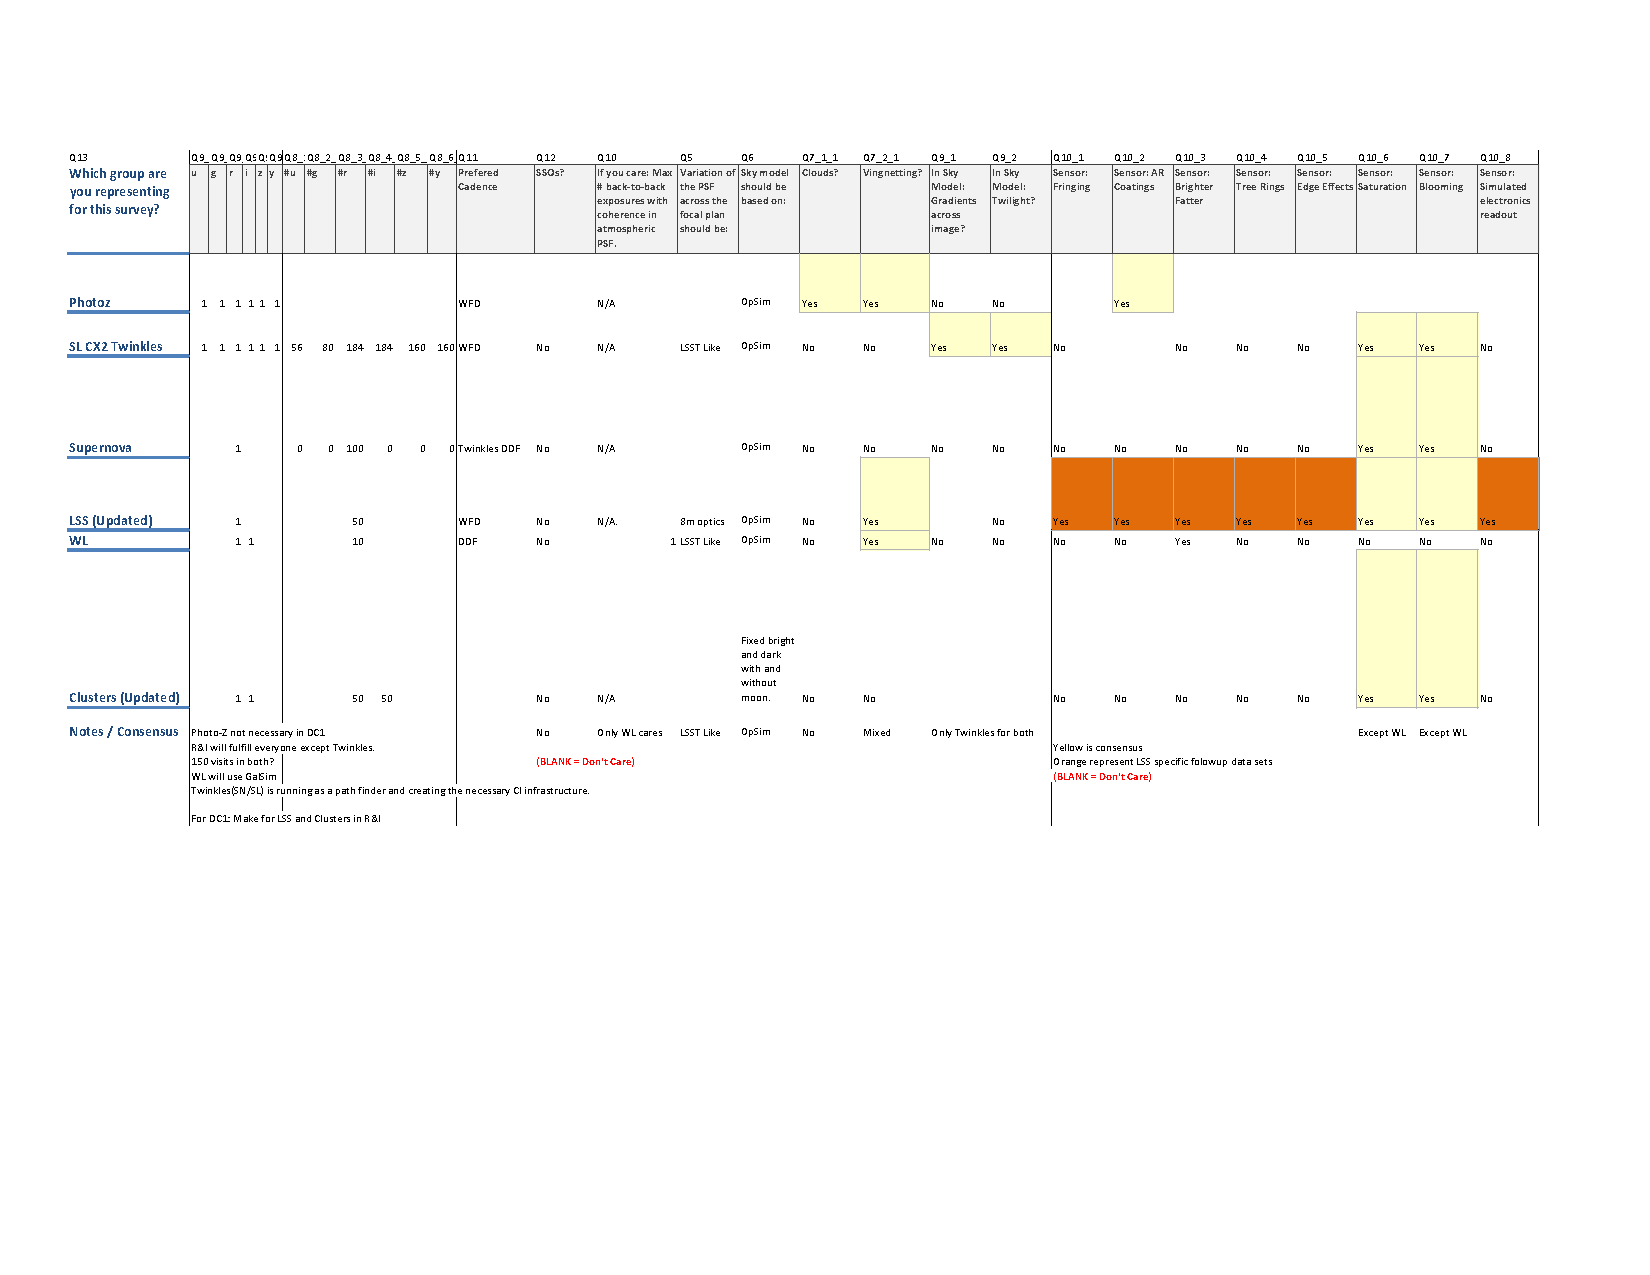
\includepdf[pages=1,angle=90]{Simulation_Requirements_Survey.pdf} 

\end{appendices}

\begin{thebibliography}{100}

\bibitem{SRM:2015} 
DESC Science Roadmap,
\url{http://lsst-desc.org/sites/default/files/DESC_SRM_V1.pdf}, 2015

\end{thebibliography}

\end{document}
